% Proofs and references: experiments/wellposedness_notes.md.
% These tanh constructions are independent of the Gaussian example in
% Zuazua, arXiv:2606.04018v2.

\renewcommand{\slideid}{L3-Q01}
\begin{frame}[c]{Question 1: is the neural minimum attained?}
\small
\guidingquestion{Even for a well-posed PDE, must a best neural-network solution exist?}
Consider the uniquely solvable problem
\[
 -u''=0\quad\text{in }(0,1),\qquad u(0)=0,\quad u(1)=1;
 \qquad u(x)=x.
\]
Fix any finite width $m\ge1$ and use a shallow tanh network:
\[
 u_\theta(x)=c+\sum_{j=1}^{m}a_j\tanh(b_jx+d_j).
\]
\[
 \Loss(v)=\int_0^1|v''(x)|^2\dd x
       +|v(0)|^2+|v(1)-1|^2.
\]
\begin{block}{Loss can approach zero without attaining it}
We will construct networks with loss tending to zero, while no finite
parameter vector attains zero loss.
\end{block}
\end{frame}

\renewcommand{\slideid}{L3-Q02}
\begin{frame}[c]{A tanh sequence approaches the infimum}
\small
One hidden neuron already gives the sequence
\[
 \boxed{v_n(x)=\frac{\tanh(x/n)}{\tanh(1/n)}},\qquad n=1,2,\ldots
\]
\[
 v_n(0)=0,\qquad v_n(1)=1,\qquad
 v_n\longrightarrow x\quad\text{in }C^2[0,1].
\]
Indeed, Taylor expansion yields
\[
 v_n(x)=x+\frac{x-x^3}{3n^2}+O(n^{-4}),\qquad
 v_n''(x)=-\frac{2x}{n^2}+O(n^{-4}).
\]
\[
 \Loss(v_n)=\frac{4}{3n^4}+O(n^{-6})\longrightarrow0.
\]
\begin{block}{The output weight diverges while the functions converge}
The output weight $a_1^{(n)}=1/\tanh(1/n)\sim n$ diverges.
The corresponding functions converge to the exact PDE solution.
\end{block}
\end{frame}

\renewcommand{\slideid}{L3-Q03}
\begin{frame}[c]{Why no finite tanh network attains this minimum}
\small
\begin{slideitems}
\item If $\Loss(u_\theta)=0$, then $u_\theta''=0$ and the endpoint data
force $u_\theta(x)=x$ throughout $(0,1)$.
\item A finite sum of tanh units is real analytic on $\R$.
Equality on an interval would therefore imply $u_\theta(x)=x$ on all of $\R$.
\item Every such finite tanh sum is bounded on $\R$; the function $x$ is
unbounded. This is a contradiction.
\end{slideitems}
\[
 \boxed{\inf_{\theta\in\Theta}\Loss(u_\theta)=0,
 \qquad \argmin_{\theta\in\Theta}\Loss(u_\theta)=\varnothing.}
\]
\begin{block}{Existence and approximation are different questions}
The PDE has a unique solution. The neural infimum is approached arbitrarily
well, but its limit lies outside this fixed finite tanh class.
\end{block}
\labnote{The conclusion depends on the stated architecture: adding a linear
skip connection makes $v(x)=x$ representable and removes this example.}
\end{frame}

\renewcommand{\slideid}{L3-Q04}
\begin{frame}[c]{Question 2: do small continuous residuals force convergence?}
\small
\guidingquestion{If $\Loss(u_{\theta_n})\to0$ for the exact integral loss, must
$u_{\theta_n}$ converge to the PDE solution in $L^2$?}
Consider the semilinear Neumann problem
\[
 -u''+\frac{u}{1+u^2}=0\quad\text{in }(0,1),
 \qquad u'(0)=u'(1)=0.
\]
Multiplying by $u$ and integrating gives
\[
 \int_0^1\left(|u'|^2+\frac{u^2}{1+u^2}\right)\dd x=0,
 \qquad\text{so the unique solution is }u=0.
\]
\begin{block}{The continuous residual loss}
\[
 \Loss(v)=\int_0^1\left|-v''+\frac{v}{1+v^2}\right|^2\dd x
             +|v'(0)|^2+|v'(1)|^2.
\]
\end{block}
\labnote{All integrals are exact. This example tests global residual-to-state stability,
without introducing sampling or quadrature.}
\end{frame}

\renewcommand{\slideid}{L3-Q05}
\begin{frame}[c]{Counterexample: vanishing continuous loss, diverging state}
\small
One tanh neuron represents a constant sequence:
\[
 v_n(x)=\frac{n}{\tanh(1)}\tanh(0x+1)=n,
 \qquad v_n'(0)=v_n'(1)=0.
\]
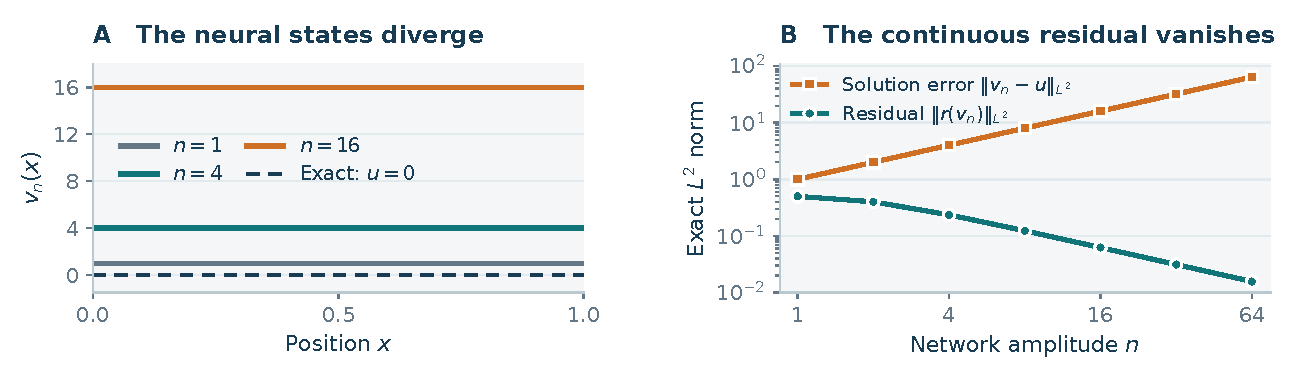
\includegraphics[width=\textwidth]{experiments/figures/continuous_residual.pdf}
\[
 \boxed{\Loss(v_n)=\frac{n^2}{(1+n^2)^2}\to0,
 \qquad \norm{v_n-u}_{L^2(0,1)}=n\to\infty.}
\]
\labnote{Uniqueness alone gives no global residual-to-error bound:
$s/(1+s^2)\to0$ as $s\to\infty$.}
\end{frame}
\renewcommand{\slideid}{L3}
